\documentclass[11pt,a4paper]{report}
\usepackage[textwidth=37em,vmargin=30mm]{geometry}
\usepackage{calc,xunicode,amsmath,amssymb,paralist,enumitem,tabu,booktabs,datetime2,xeCJK,xeCJKfntef,listings}
\usepackage{tocloft,fancyhdr,tcolorbox,xcolor,graphicx,eso-pic,xltxtra,xelatexemoji}

\newcommand{\envyear}[0]{2025}
\newcommand{\envdatestr}[0]{2025-06-25}
\newcommand{\envfinaldir}[0]{webdb/2025/20250625/final}

\usepackage[hidelinks]{hyperref}
\hypersetup{
    colorlinks=false,
    pdfpagemode=FullScreen,
    pdftitle={Web Digest - \envdatestr}
}

\setlength{\cftbeforechapskip}{10pt}
\renewcommand{\cftchapfont}{\rmfamily\bfseries\large\raggedright}
\setlength{\cftbeforesecskip}{2pt}
\renewcommand{\cftsecfont}{\sffamily\small\raggedright}

\setdefaultleftmargin{2em}{2em}{1em}{1em}{1em}{1em}

\usepackage{xeCJK,xeCJKfntef}
\xeCJKsetup{PunctStyle=plain,RubberPunctSkip=false,CJKglue=\strut\hskip 0pt plus 0.1em minus 0.05em,CJKecglue=\strut\hskip 0.22em plus 0.2em}
\XeTeXlinebreaklocale "zh"
\XeTeXlinebreakskip = 0pt


\setmainfont{Brygada 1918}
\setromanfont{Brygada 1918}
\setsansfont{IBM Plex Sans}
\setmonofont{JetBrains Mono NL}
\setCJKmainfont{Noto Serif CJK SC}
\setCJKromanfont{Noto Serif CJK SC}
\setCJKsansfont{Noto Sans CJK SC}
\setCJKmonofont{Noto Sans CJK SC}

\setlength{\parindent}{0pt}
\setlength{\parskip}{8pt}
\linespread{1.15}

\lstset{
	basicstyle=\ttfamily\footnotesize,
	numbersep=5pt,
	backgroundcolor=\color{black!5},
	showspaces=false,
	showstringspaces=false,
	showtabs=false,
	tabsize=2,
	captionpos=b,
	breaklines=true,
	breakatwhitespace=true,
	breakautoindent=true,
	linewidth=\textwidth
}






\newcommand{\coverpic}[2]{
    % argv: itemurl, authorname
    Cover photo by #2~~(\href{#1}{#1})
}
\newcommand{\makeheader}[0]{
    \begin{titlepage}
        % \newgeometry{hmargin=15mm,tmargin=21mm,bmargin=12mm}
        \begin{center}
            
            \rmfamily\scshape
            \fontspec{BaskervilleF}
            \fontspec{Old Standard}
            \fontsize{59pt}{70pt}\selectfont
            WEB\hfill DIGEST
            
            \vfill
            % \vskip 30pt
            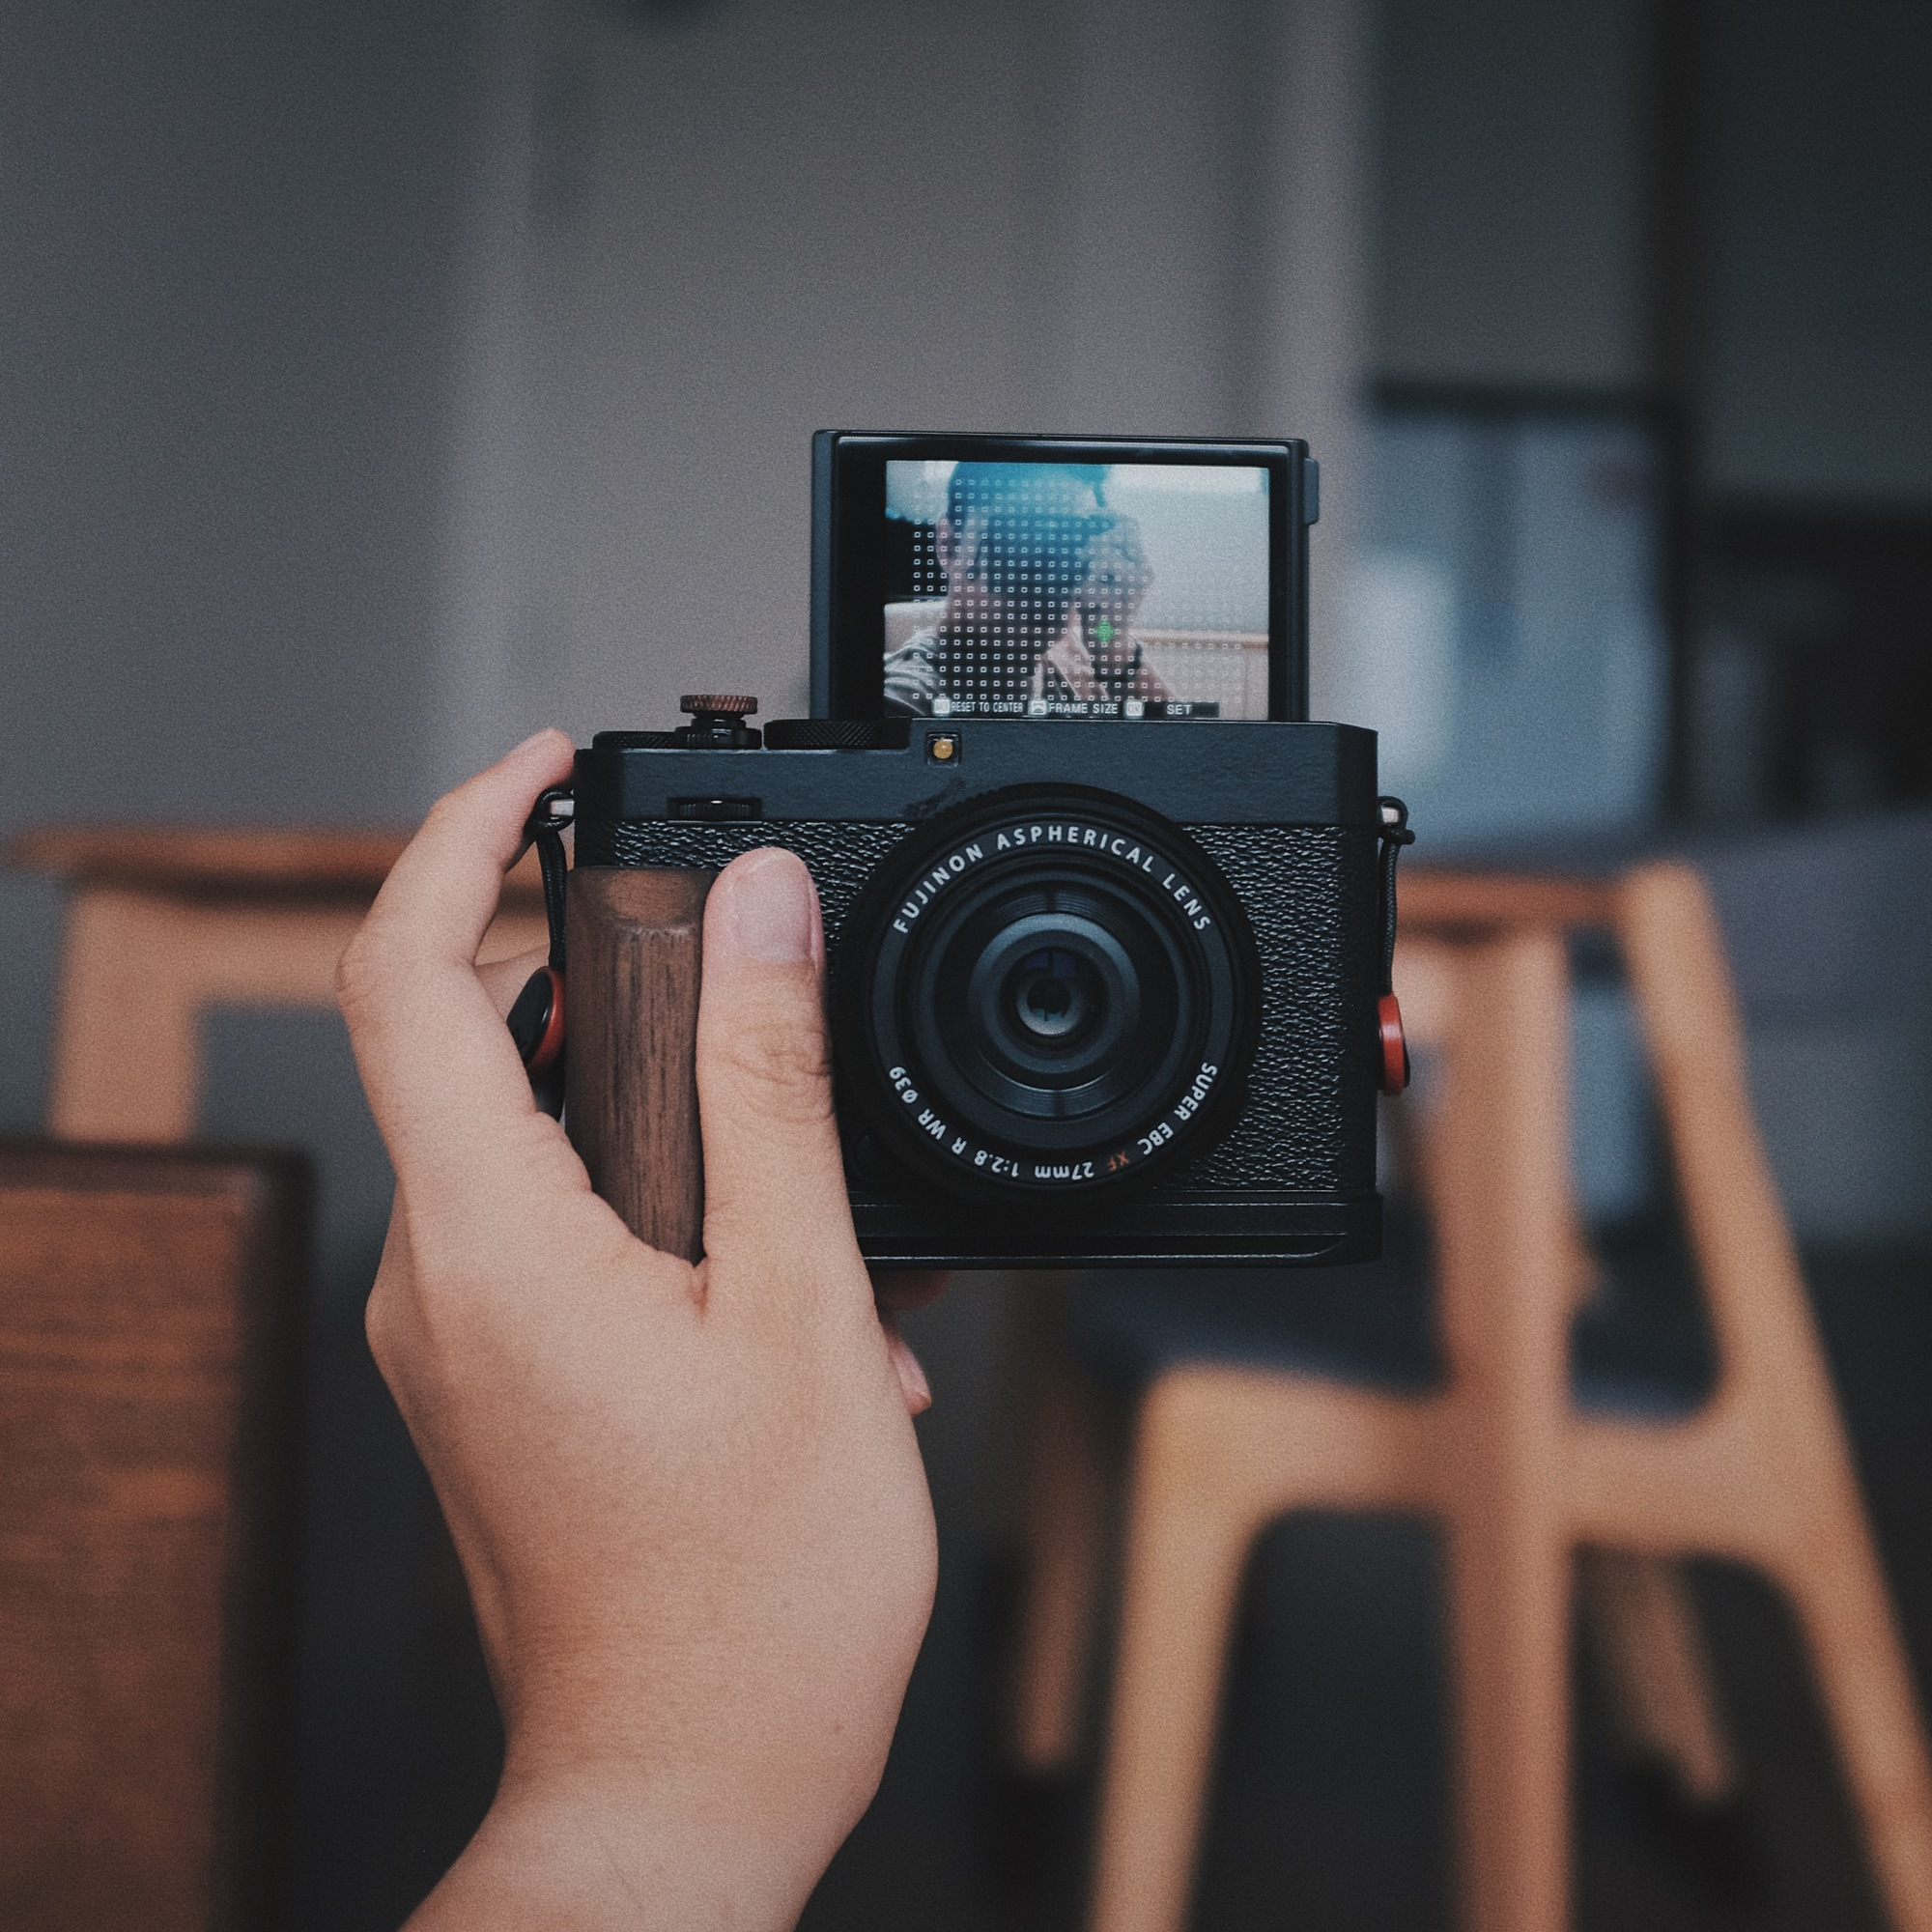
\includegraphics[width=\linewidth]{\envfinaldir/coverpic-prod.jpg}\par
            % \vskip 30pt
            \vfill

            \normalsize\rmfamily\scshape
            \copyright{} The Web Digest Project \hfill\large \envdatestr
        \end{center}
    \end{titlepage}
    % \restoregeometry
}
\newcommand{\simplehref}[1]{%
    \textcolor{blue!80!green}{\href{#1}{#1}}%
}
\renewcommand{\contentsname}{\center\Huge\sffamily\bfseries Contents\par\vskip 20pt}
\newcounter{ipartcounter}
\setcounter{ipartcounter}{0}
\newcommand{\ipart}[1]{
    % \vskip 20pt
    \clearpage
    \stepcounter{ipartcounter}
    \phantomsection
    \addcontentsline{toc}{chapter}{#1}
    % \begin{center}
    %     \Huge
    %     \sffamily\bfseries
    %     #1
    % \end{center}
    % \vskip 20pt plus 7pt
}
\newcounter{ichaptercounter}
\setcounter{ichaptercounter}{0}
\newcommand{\ichapter}[1]{
    % \vskip 20pt
    \clearpage
    \stepcounter{ichaptercounter}
    \phantomsection
    \addcontentsline{toc}{section}{\numberline{\arabic{ichaptercounter}}#1}
    \begin{center}
        \Huge
        \sffamily\bfseries
        #1
    \end{center}
    \vskip 20pt plus 7pt
}
\newcommand{\entrytitlefont}[1]{\subsection*{\raggedright\Large\sffamily\bfseries#1}}
\newcommand{\entryitemGeneric}[2]{
    % argv: title, url
    \parbox{\linewidth}{
        \entrytitlefont{#1}\par\vskip 5pt
        \footnotesize\ttfamily\mdseries
        \simplehref{#2}
    }\vskip 11pt plus 11pt minus 1pt
}
\newcommand{\entryitemGithub}[3]{
    % argv: title, url, desc
    \parbox{\linewidth}{
        \entrytitlefont{#1}\par\vskip 5pt
        \footnotesize\ttfamily\mdseries
        \simplehref{#2}\par\vskip 5pt
        \small\rmfamily\mdseries#3
    }\vskip 11pt plus 11pt minus 1pt
}
\newcommand{\entryitemAp}[3]{
    % argv: title, url, desc
    \parbox{\linewidth}{
        \entrytitlefont{#1}\par\vskip 5pt
        \footnotesize\ttfamily\mdseries
        \simplehref{#2}\par\vskip 5pt
        \small\rmfamily\mdseries#3
    }\vskip 11pt plus 11pt minus 1pt
}
\newcommand{\entryitemHackernews}[3]{
    % argv: title, hnurl, rawurl
    % \parbox{\linewidth}{
    %     \entrytitlefont{#1}\par\vskip 5pt
    %     \footnotesize\ttfamily\mdseries
    %     \simplehref{#3}\par
    %     \textcolor{black!50}{\href{#2}{#2}}
    % }\vskip 11pt plus 11pt minus 1pt
    \begin{minipage}{\linewidth}
            \entrytitlefont{#1}\par\vskip 5pt
            \footnotesize\ttfamily\mdseries
            \simplehref{#3}\par
            \textcolor{black!50}{\href{#2}{#2}}
    \end{minipage}\par\vskip 11pt plus 11pt minus 1pt
}







\begin{document}

\makeheader

\tableofcontents\clearpage




\ipart{Developers}
\ichapter{Hacker News}
\entryitemTwoLinks{National Archives to restrict public access starting July 7}{https://news.ycombinator.com/item?id=44371169}{https://www.archives.gov/college-park}

\entryitemTwoLinks{Ancient X11 scaling technology}{https://news.ycombinator.com/item?id=44369646}{https://flak.tedunangst.com/post/forbidden-secrets-of-ancient-X11-scaling-technology-revealed}

\entryitemTwoLinks{Fun with uv and PEP 723}{https://news.ycombinator.com/item?id=44369388}{https://www.cottongeeks.com/articles/2025-06-24-fun-with-uv-and-pep-723}

\entryitemTwoLinks{Man 'refused entry into US' as border control catch him with bald JD Vance meme}{https://news.ycombinator.com/item?id=44369140}{https://www.dublinlive.ie/news/world-news/man-refused-entry-us-border-31925059}

\entryitemTwoLinks{iPhone customers upset by Apple Wallet ad pushing F1 movie}{https://news.ycombinator.com/item?id=44368854}{https://techcrunch.com/2025/06/24/iphone-customers-upset-by-apple-wallet-ad-pushing-f1-movie/}

\entryitemTwoLinks{A federal judge sides with Anthropic in lawsuit over training AI on books}{https://news.ycombinator.com/item?id=44367850}{https://techcrunch.com/2025/06/24/a-federal-judge-sides-with-anthropic-in-lawsuit-over-training-ai-on-books-without-authors-permission/}

\entryitemTwoLinks{ChatGPT's enterprise success against Copilot fuels OpenAI/Microsoft rivalry}{https://news.ycombinator.com/item?id=44367638}{https://www.bloomberg.com/news/articles/2025-06-24/chatgpt-vs-copilot-inside-the-openai-and-microsoft-rivalry}

\entryitemTwoLinks{XBOW, an autonomous penetration tester, has reached the top spot on HackerOne}{https://news.ycombinator.com/item?id=44367548}{https://xbow.com/blog/top-1-how-xbow-did-it/}

\entryitemTwoLinks{Writing toy software is a joy}{https://news.ycombinator.com/item?id=44367084}{https://blog.jsbarretto.com/post/software-is-joy}

\entryitemTwoLinks{Nordic Semiconductor Acquires Memfault}{https://news.ycombinator.com/item?id=44367071}{https://www.nordicsemi.com/Nordic-news/2025/06/Nordic-Semiconductor-acquires-Memfault}

\entryitemTwoLinks{PlasticList – Plastic Levels in Foods}{https://news.ycombinator.com/item?id=44366548}{https://www.plasticlist.org/}

\entryitemTwoLinks{The bitter lesson is coming for tokenization}{https://news.ycombinator.com/item?id=44366494}{https://lucalp.dev/bitter-lesson-tokenization-and-blt/}

\entryitemTwoLinks{Gemini Robotics On-Device brings AI to local robotic devices}{https://news.ycombinator.com/item?id=44366409}{https://deepmind.google/discover/blog/gemini-robotics-on-device-brings-ai-to-local-robotic-devices/}

\entryitemTwoLinks{Finding a 27-year-old easter egg in the Power Mac G3 ROM}{https://news.ycombinator.com/item?id=44365806}{https://www.downtowndougbrown.com/2025/06/finding-a-27-year-old-easter-egg-in-the-power-mac-g3-rom/}

\entryitemTwoLinks{Basic Facts about GPUs}{https://news.ycombinator.com/item?id=44365320}{https://damek.github.io/random/basic-facts-about-gpus/}

\entryitemTwoLinks{SourceHut moves business operations from US to Europe}{https://news.ycombinator.com/item?id=44365246}{https://lists.sr.ht/~sircmpwn/sr.ht-dev/patches/60282}

\entryitemTwoLinks{Starship: The minimal, fast, and customizable prompt for any shell}{https://news.ycombinator.com/item?id=44364874}{https://starship.rs/}

\entryitemTwoLinks{A Mysterious Website I Stumbled Upon}{https://news.ycombinator.com/item?id=44364667}{https://www.sbnation.com/a/17776-football}

\entryitemTwoLinks{Microplastics shed by food packaging are contaminating our food, study finds}{https://news.ycombinator.com/item?id=44364526}{https://www.cnn.com/2025/06/24/health/microplastics-food-packaging-study-wellness}

\entryitemTwoLinks{Switching Pip to Uv in a Dockerized Flask / Django App}{https://news.ycombinator.com/item?id=44364406}{https://nickjanetakis.com/blog/switching-pip-to-uv-in-a-dockerized-flask-or-django-app}


\ipart{Developers~~~~(zh-Hans)}
\ichapter{Solidot}
\entryitemGeneric{\hskip 0pt{}中国五月份太阳能装机容量创下新记录}{https://www.solidot.org/story?sid=81639}

\entryitemGeneric{\hskip 0pt{}Vera C. Rubin 天文台公布了首批宇宙全景照}{https://www.solidot.org/story?sid=81638}

\entryitemGeneric{\hskip 0pt{}Google Chromebook 笔记本电脑集成 AI 功能}{https://www.solidot.org/story?sid=81637}

\entryitemGeneric{\hskip 0pt{}亚马逊加速发射互联网宽带卫星}{https://www.solidot.org/story?sid=81636}

\entryitemGeneric{\hskip 0pt{}IYO 就 IO 商标起诉 OpenAI}{https://www.solidot.org/story?sid=81635}

\entryitemGeneric{\hskip 0pt{}Firefox 140 释出}{https://www.solidot.org/story?sid=81634}

\entryitemGeneric{\hskip 0pt{}玻璃瓶瓶盖显著增加了饮料中的微塑料含量}{https://www.solidot.org/story?sid=81633}

\entryitemGeneric{\hskip 0pt{}博士数量超过学界需求}{https://www.solidot.org/story?sid=81632}

\entryitemGeneric{\hskip 0pt{}马斯克现身YC大会:谈``智能大爆炸''时代的生存法则,结合PayPal、SpaceX、特斯拉、xAI创业史,详解如何使用第一性原理}{https://www.solidot.org/story?sid=81631}

\entryitemGeneric{\hskip 0pt{}微软设定 Windows 11 系统还原点的有效时间为 60 天}{https://www.solidot.org/story?sid=81630}

\entryitemGeneric{\hskip 0pt{}一颗死亡的 NASA 卫星突然发射出强大的射电信号}{https://www.solidot.org/story?sid=81629}

\entryitemGeneric{\hskip 0pt{}分析师认为 AI 没有做好它的工作}{https://www.solidot.org/story?sid=81628}

\entryitemGeneric{\hskip 0pt{}减肥显著提升一个人的自尊水平}{https://www.solidot.org/story?sid=81627}

\entryitemGeneric{\hskip 0pt{}AI 如何影响印度的呼叫中心行业}{https://www.solidot.org/story?sid=81626}

\entryitemGeneric{\hskip 0pt{}Bill Gates 和 Linus Torvalds 首次同框}{https://www.solidot.org/story?sid=81625}

\entryitemGeneric{\hskip 0pt{}Kubuntu 移除对 X11 的默认支持}{https://www.solidot.org/story?sid=81624}

\entryitemGeneric{\hskip 0pt{}食品广告如何影响儿童体重}{https://www.solidot.org/story?sid=81623}

\entryitemGeneric{\hskip 0pt{}Cursor 的开源替代 Void IDE 发布 Beta 版本}{https://www.solidot.org/story?sid=81622}

\entryitemGeneric{\hskip 0pt{}有经验 FPS 玩家的瞄准优势在于其更快的执行时间}{https://www.solidot.org/story?sid=81621}

\entryitemGeneric{\hskip 0pt{}三星在西亚北非出售的手机中预装了以色列软件 AppCloud}{https://www.solidot.org/story?sid=81620}\ichapter{V2EX}
\entryitemGeneric{\hskip 0pt{}[推广] vibecoding 了一个高流量低竞争的 Asphalt Calculator}{https://www.v2ex.com/t/1140791}

\entryitemGeneric{\hskip 0pt{}[分享创造] 随手写了个 couponclip.it.com 优惠价 AI 管家}{https://www.v2ex.com/t/1140790}

\entryitemGeneric{\hskip 0pt{}[宽带症候群] Nas 上 qBittorrent 在多 Wan 拨号情况下,外部 IP 非本机地址而是 Lan 接口地址是为什么}{https://www.v2ex.com/t/1140789}

\entryitemGeneric{\hskip 0pt{}[分享创造] TA-Box:纯 Python 实现的 TA-Lib 替代方案}{https://www.v2ex.com/t/1140788}

\entryitemGeneric{\hskip 0pt{}[问与答] 最近抖音很火的``差点忘了以前是干嘛的''系列,是不是证明年轻人的出路只有一条就是做抖音主播?}{https://www.v2ex.com/t/1140787}

\entryitemGeneric{\hskip 0pt{}[Windows] 微软宣布 Windows 10 延长更新服务将``免费''向用户提供}{https://www.v2ex.com/t/1140786}

\entryitemGeneric{\hskip 0pt{}[问与答] 医疗保险求推荐哪家靠谱}{https://www.v2ex.com/t/1140785}

\entryitemGeneric{\hskip 0pt{}[程序员] cloudflare containers 来了, 真不错}{https://www.v2ex.com/t/1140784}

\entryitemGeneric{\hskip 0pt{}[摄影] 有什么好相机推荐?我做这份表格,欢迎老手指点}{https://www.v2ex.com/t/1140783}

\entryitemGeneric{\hskip 0pt{}[程序员] XXL-JOB v3.1.1 | 分布式任务调度平台(Dify 工作流调度增强)}{https://www.v2ex.com/t/1140782}

\entryitemGeneric{\hskip 0pt{}[宽带症候群] 怎么从路由器上屏蔽抖音和微信视频号?}{https://www.v2ex.com/t/1140781}

\entryitemGeneric{\hskip 0pt{}[分享发现] 现在的 AI 除了生成视频,还能同步生成语音了?}{https://www.v2ex.com/t/1140780}

\entryitemGeneric{\hskip 0pt{}[分享发现] ElevenLabs 推出了一款名为 11ai 的 AI 个人助理,可以用来免费练英语口语。}{https://www.v2ex.com/t/1140779}

\entryitemGeneric{\hskip 0pt{}[Android] ColorOS 怎么实现微信语音自动录音?}{https://www.v2ex.com/t/1140778}

\entryitemGeneric{\hskip 0pt{}[职场话题] 浅谈毕业找工作这件事(观毕业迷茫贴有感)}{https://www.v2ex.com/t/1140777}

\entryitemGeneric{\hskip 0pt{}[问与答] 自动生成企业 logo 和名片,有推荐的站点吗?}{https://www.v2ex.com/t/1140776}

\entryitemGeneric{\hskip 0pt{}[虚拟现实] 2025 年中了, vision pro 有哪些有意思的软件?}{https://www.v2ex.com/t/1140775}

\entryitemGeneric{\hskip 0pt{}[程序员] 如何快速学习 riscv 版的 FreeRTOS?}{https://www.v2ex.com/t/1140774}

\entryitemGeneric{\hskip 0pt{}[Android] 国产手机的浏览器是同一家公司开发的吗?}{https://www.v2ex.com/t/1140773}

\entryitemGeneric{\hskip 0pt{}[问与答] miniMax TTS 是不是刷排行榜了?}{https://www.v2ex.com/t/1140772}

\entryitemGeneric{\hskip 0pt{}[随想] 避雷 4k-nf}{https://www.v2ex.com/t/1140771}

\entryitemGeneric{\hskip 0pt{}[分享创造] 又又又一个 yt-dlp 包装的 Mac 音乐播放器,不过这次有点不一样~}{https://www.v2ex.com/t/1140769}

\entryitemGeneric{\hskip 0pt{}[问与答] 30 岁这个弯要怎么转,背贷款买房 or 回家车房老婆热炕头}{https://www.v2ex.com/t/1140768}

\entryitemGeneric{\hskip 0pt{}[问与答] 和特斯拉相关的哪些有意思的项目}{https://www.v2ex.com/t/1140767}

\entryitemGeneric{\hskip 0pt{}[分享创造] 做了一个 chrome 插件,查看 AI 对话大纲}{https://www.v2ex.com/t/1140766}

\entryitemGeneric{\hskip 0pt{}[问与答] 最近云完《捞女游戏》,很好奇大家现实生活中遇到过捞女么}{https://www.v2ex.com/t/1140765}

\entryitemGeneric{\hskip 0pt{}[程序员] 发布一个隐私优先视频分析工具 - VidLoad.cc}{https://www.v2ex.com/t/1140764}

\entryitemGeneric{\hskip 0pt{}[分享创造] 写了一个通过大语言模型 LLM 解读最新 arXiv 论文的 Github 项目,不知道有没有用?}{https://www.v2ex.com/t/1140762}

\entryitemGeneric{\hskip 0pt{}[Kotlin] Kotlin 中文文档 2.1.20 版翻译完成了}{https://www.v2ex.com/t/1140761}

\entryitemGeneric{\hskip 0pt{}[游戏] steam 文明 6 大促, 220 -> 11}{https://www.v2ex.com/t/1140760}

\entryitemGeneric{\hskip 0pt{}[PayPal] 出 paypal1050\$}{https://www.v2ex.com/t/1140759}

\entryitemGeneric{\hskip 0pt{}[生活] 发现夏洛和树先生很像}{https://www.v2ex.com/t/1140757}

\entryitemGeneric{\hskip 0pt{}[问与答] 求推荐一个扫描仪 600ppi 彩色双面带 ADF}{https://www.v2ex.com/t/1140756}

\entryitemGeneric{\hskip 0pt{}[程序员] 推荐一款很装又实用的编程字体}{https://www.v2ex.com/t/1140755}

\entryitemGeneric{\hskip 0pt{}[汽车] 买车推荐了}{https://www.v2ex.com/t/1140754}

\entryitemGeneric{\hskip 0pt{}[音乐] 300 元内有啥小尾巴可以推荐吗?新的二手的都可以}{https://www.v2ex.com/t/1140751}

\entryitemGeneric{\hskip 0pt{}[VPS] vps 快到期了,哪家稳定不被封}{https://www.v2ex.com/t/1140750}

\entryitemGeneric{\hskip 0pt{}[Apple] iPhone 重装系统激活时不选择还原 icloud 备份,进系统后,能恢复 icloud 中的相册和其他数据吗}{https://www.v2ex.com/t/1140749}

\entryitemGeneric{\hskip 0pt{}[分享发现] 香港银联信用卡-大润发付 50 减 20}{https://www.v2ex.com/t/1140748}

\entryitemGeneric{\hskip 0pt{}[问与答] "小小电脑"不能玩键盘游戏?}{https://www.v2ex.com/t/1140747}

\entryitemGeneric{\hskip 0pt{}[Telegram] giffgaff 分配的手机号都被注册过 telegram 了}{https://www.v2ex.com/t/1140746}

\entryitemGeneric{\hskip 0pt{}[Android] lineageos 的 ipv6 是不是有问题}{https://www.v2ex.com/t/1140745}

\entryitemGeneric{\hskip 0pt{}[程序员] [诈骗页面] 绩效补贴页面功能升级了,带 debugger 调试监测,代码也加密了。}{https://www.v2ex.com/t/1140743}

\entryitemGeneric{\hskip 0pt{}[酷工作] Airbnb 中国内推}{https://www.v2ex.com/t/1140742}

\entryitemGeneric{\hskip 0pt{}[问与答] vivo 的地震数据更新是不是有问题?}{https://www.v2ex.com/t/1140741}

\entryitemGeneric{\hskip 0pt{}[问与答] [讨论] 官方:个人养老金领取时需缴个税}{https://www.v2ex.com/t/1140740}

\entryitemGeneric{\hskip 0pt{}[职场话题] 进入职场后是不是只区分优等 985 本科 专科}{https://www.v2ex.com/t/1140739}

\entryitemGeneric{\hskip 0pt{}[问与答] 如何主动失信,成为黑户。不能网贷借钱}{https://www.v2ex.com/t/1140738}

\entryitemGeneric{\hskip 0pt{}[全球工单系统] frp 的单进程模型}{https://www.v2ex.com/t/1140736}

\entryitemGeneric{\hskip 0pt{}[酷工作] [组内直推-高级算法工程师]滴滴出行-两轮车事业部}{https://www.v2ex.com/t/1140735}


\ipart{Generic News}







\clearpage
\leavevmode\vfill
\footnotesize

Copyright \copyright{} 2023-2025 Neruthes and other contributors.

This document is published with CC BY-NC-ND 4.0 license.

The entries listed in this newsletter may be copyrighted by their respective creators.

This newsletter is generated by the Web Digest project.

The newsletters are also delivered via Telegram channel \CJKunderline{\href{https://t.me/webdigestchannel}{https://t.me/webdigestchannel}}.\\
RSS feed is available at \CJKunderline{\href{https://webdigest.pages.dev/rss.xml}{https://webdigest.pages.dev/rss.xml}}.

This newsletter is available in PDF at
\CJKunderline{\href{https://webdigest.pages.dev/}{https://webdigest.pages.dev/}}.

The source code being used to generate this newsletter is available at\\
\CJKunderline{\href{https://github.com/neruthes/webdigest}{https://github.com/neruthes/webdigest}}.

This newsletter is also available in
\CJKunderline{\href{http://webdigest.pages.dev/readhtml/\envyear/WebDigest-20250625.html}{HTML}} and
\CJKunderline{\href{https://github.com/neruthes/webdigest/blob/master/markdown/\envyear/WebDigest-20250625.md}{Markdown}}.


\coverpic{https://unsplash.com/photos/two-colorful-doors-on-a-charming-old-building-aVMA8R054A0}{Clark Van Der Beken}


\end{document}
